\documentclass[conference]{IEEEtran}
% If the IEEEtran.cls has not been installed into the LaTeX system files,
% manually specify the path to it.  e.g.
% \documentclass[conference]{./IEEEtran}

% Add and required packages here
\usepackage{graphicx,times,amsmath,amssymb,epstopdf,algorithmicx,algpseudocode,algorithm,color,pgfplots,footnote}

% Correct bad hyphenation here
\hyphenation{perpen-dicular}

% To create the author's affliation portion using \thanks
\IEEEoverridecommandlockouts

\textwidth 178mm
\textheight 239mm
\oddsidemargin -7mm
\evensidemargin -7mm
\topmargin -6mm
\columnsep 5mm

% Vector shorthand.
\newcommand{\vect}[2]{\ensuremath{\Bigl(\negthinspace\begin{smallmatrix}#1\\#2\end{smallmatrix}}\Bigr)}

\begin{document}

% Project title: keep the \ \\ \LARGE\bf in it to leave enough margin.
\title{\ \\ \LARGE\bf MAIG Group Project \\ Monte-Carlo Tree Search in TORCS}

\author{Jacob Fischer (jaco@itu.dk), Nikolaj Falsted (nifa@itu.dk) \& Mathias Vielwerth (mvie@itu.dk)}

% Make the title area
\maketitle

\thispagestyle{plain}
\pagestyle{plain}

\begin{abstract}
Tree search methods are rarely applied in the effort to control racing cars with artifical intelligence, as such an approach first requires the development of an efficient and fairly accurate forward model. This paper details our approach to this challenge, where we have applied the Monte-Carlo Tree Search method to the open-source racing simulator TORCS. 

A functioning and efficient forward model was developed, consisting of a number of sub-tasks capable of constructing it, transforming to it and simulating in it. This framework allows a tree-search based racing controller to make use of the Monte-Carlo method for best-first search decision-making in a discretized action space, where an action is represented by pressure on the gas pedal and rotation of the steering wheel.

We conclude that it is possible to implement an able racing controller based on this method, which generalizes to most road tracks as long as a warm-up period is provided. Deficiencies of the forward model, however, prevent it from competing on certain tracks.
\end{abstract}

\section{Introduction}
\PARstart{C}{ar} racing games present an interesting challenge in the field of artificial intelligence. It is a difficult domain in which to achieve a competent skill-level for computer controlled agents, being characterized by a wide, continuous action space, real-time decision making, and the need for at least some level of foresight if optimal play is desired. In addition, scientific progress here can have potential application outside of games, with an evident parallel to autonomous cars.

The Open Car Racing Simulator (TORCS) is an oft-used platform for experimenting with different approaches to AI in car racing. A deal of academic research has been produced \cite{optimalraceline}\cite{trackmodel}\cite{cobostar}\cite{fluff} with TORCS as the platform for trying out novel solutions to the problem of AI-controlled racing cars. A scientific competition is held annually under IEEE auspices \cite{2008championship}\cite{2009championship}, which provides a set of rules that levels the playing field between potential solutions, as well as a programmatic client-server framework that enforces these rules.

Most prevalent in the competition are solutions involving artificial neural networks (ANNs), genetic algorithms or a combination of these two. Planning algorithms in general, but tree search methods in particular seem very under-represented, making it an ideal avenue to explore. Furthermore, the sensory character of ANNs means that they usually lack foresight, and are inherently difficult to generalize across different tracks. A planning-based method seems a natural candidate for approaching the problem from a different angle.

Monte-Carlo Tree Search (MCTS) is a best-first search method that builds a search tree iteratively, and bases its decision making in statistical analysis of simulated play-outs \cite{browne}. It has received significant attention for its ability to make “educated guesses” in situations where the search space is too large for exhaustive search methods to be applicable. MCTS received its initial breakthrough showing significant potential in turn-based games such as Go \cite{go} and Hex \cite{hex}. It has since been adapted to real-time applications as well \cite{pacman}, but racing games do not seem to be among them.

Moved by the lack of research on the application of planning algorithms to AI in TORCS, and inspired by the recent successes of (and perhaps a personal, slightly unhealthy infatuation with) Monte-Carlo Tree Search, we will in this article present our findings, having successfully produced a car racing controller that makes its decisions exclusively based on tree search with simulated playouts. The goal of this article lies not in creating a competition-winning car controller, but rather examining the usage of planning algorithms, specifically MCTS, in racing games. TORCS and the competition framework is used for its convenience, and results are compared to competition results as a general measure of utility.

In order to apply any tree search method to an AI, two things are needed: a forward model capable of predicting future game states based on what actions are taken, and an evaluation function to probe the desirability of a given game state. Under the competition framework, we only have access to data that is relative to the car's position on the racing track at any given time step, which is not sufficient for simulating future time steps, requiring static knowledge of the track's shape. The rules of the competition \cite{manual} allow for a warm-up period before the race, which we utilize to record the track in advance.

Furthermore, the sensor state space mapped out by this data is not Euclidean \cite{euclidean}, making it less ideal for applying a forward model intended to approximate a car racing physics engine. Hence, we map the recorded data of the track to a 2-dimensional Euclidean space, and a vector based forward model implemented by deference to the laws of classical physics is used to simulate play-outs.

Section \ref{sec-method} will examine how Monte-Carlo Tree Search can be used to control a car in TORCS, assuming an accurate forward model is given. Then, we will explain our approach to providing such a forward model, focusing on the three essential parts of this endeavor (section \ref{sec-model}):
\begin{itemize}
\item Recording the track during warm-up and mapping it to a Euclidean space
\item Transforming any given state between the sensor space and the Euclidean space (and back)
\item Simulating play-outs with a vector based forward model representing a simplification of the internal engine
\end{itemize}

\section {Previous Work}
\label{sec-background}
In racing, a race line \cite{raceline} is a path along the track that a driver may follow to complete it. Finding the optimal race line in TORCS has been attained by Cardamone et al. by applying a genetic algorithm to data read from the internal track files \cite{optimalraceline}. This is used to great success, beating the allegedly best controller ``Simplix” \cite{simplix}. The one limitation of this approach, however, is that the competition does not give direct access to the track files. All the same, it highlights the strength of having a controller that is knowledgeable about the shape of the track ahead of it, allowing it to optimize the path it will follow.

Quadflieg et al. has successfully created a model of the track strictly from sensor data \cite{trackmodel}, arguing that having knowledge of the track available can pave the way for a wider application of planning algorithms. Our own track construction algorithm takes inspiration from their success, but for the simulated playouts of MCTS we had to build for ourselves a more detailed model than their method could provide.

Research into modelling a forward function has been done by Butz et al. \cite{cobostar}. Here, its application is directly in the sensor space and not combined with a track model, which limits its use with regards to planning, and in particular with regards to a tree search in the space of the car’s planar positioning. It does, however, make for an interesting comparison between utilizing a learned forward model and using a physics-based abstraction of the internal engine, such as we have done in our case.

\section{Monte-Carlo Method}
\label{sec-method}
\subsection{Tree Search Car Controller}
The \emph{tick} or time step under the competition framework is a mere 20 milliseconds long \cite{manual}. This makes sure the car is updated with a relevant view of the game world fairly often, but it also puts a limit on the runtime of the decision-making algorithm.

Monte-Carlo Tree Search is not exhaustive, and can be polled for an answer after any number of iterations. The longer it gets to run, however, the more likely it is to converge on an optimal solution. For this reason, we have designed our tree search controller to cache its search between ticks, making its decisions within an extended time interval. The car controller will record the current state at time $t$, and apply the forward model once to obtain a state at time $t+t_{step}$, where $t_{step}$ is the configurable decision time step. While driving towards this state in-game by repeatedly applying the best decision from the previous search, the controller will utilize its time budget searching for a decision from $t+t_{step}$.

In addition, utilizing tree search is intended as a mechanism for planning ahead, so it is natural that our approach involves a longer period of time between the steps at which new decisions are considered. In other words, a good decision should not have to be reconsidered immediately.

\subsection{Action Space}
An action in TORCS allows the control of a number of factors, but we have limited these to acceleration, braking and steering. Transmission is controlled by a deterministic algorithm based on RPM, and acceleration/braking is further reduced to a single value \emph{gas} for simplicity, with a negative sign representing brake.

We thus define an action as the combination of only two values: one representing gas or brake pressure, and one describing steering. Both are continuous values, and so are discretized in the interest of having as small a branching factor as possible. The average number of actions available from all states equals the average branching factor of the search tree. A smaller branching factor is always preferable, as long as the available actions allow for optimal play. Deciding which actions are needed for optimal play is not trivial, and is one of the many factors that can be tweaked (see section \ref{sec-discussion}, table \ref{tab-config}) to increase performance.

We discretize both gas pressure and steering into intervals and allow only selection of neighbouring values to the previous action. E.g. with a current gas pressure of 0.4 and an interval of 0.2, it will only be possible to take actions with a gas pressure of either 0.2, 0.4 or 0.6. This method of filtering allows for a finer granularity, while still having a low branching factor, but at the cost of being able to make sudden changes in action. In that sense, having only neighbouring actions available seems very natural and also serves as a way of reducing skidding, which is currently not modelled in our forward function. We also do not allow braking and steering at the same time, as this almost always leads to skidding.

\subsection{Evaluation Function}
Equation (\ref{eqn-eval}) displays the formula we use for evaluating the desirability of a given state. Our state space does not contain successful terminal states, since our benchmark (see section \ref{sec-results}) is based on getting as far as possible within an unlimited number of laps. Unsuccessful terminal states (denoted $\bot$) occur when the car is outside the boundaries of the track.

Our aim was for values to fall within the range $[0;1]$. A heuristic that normalizes the distance travelled along the track line by the total length of the track is not ideal, since this yields values that grow increasingly larger as the game progresses. The $C_P$ constant of the UCT formula \cite{browne}, which weighs exploration vs. exploitation in the Monte-Carlo tree search, has to be configured based on the interval of the value range. Thus, the formula in equation (\ref{eqn-eval}) yields a value relative to the \emph{local} outset of the search. 0 means the car has been motionless for the full duration of the time difference $t$ between the local outset and the current state. 1 means the car has accelerated as much as possible, following the track line perfectly for the full duration. The intention is for the heuristic to be admissible, i.e. never overestimating the theoretical maximum, which is bounded by the maximum acceleration $a_{max}$. Since the distance is measured along the middle of the track, however, and not along the optimal race line \cite{raceline}, we cannot make this claim.

\begin{equation}
\begin{alignedat}{1}
\label{eqn-eval}
& k = \frac{d - d_0}{\frac{1}{2}a_{max}t^2 + v_0t} \\
& k_\bot = k^2 * P
\end{alignedat}
\end{equation}
where $d$ is the distance along the track line in the given state, $d_0$ is the distance along the track in the state at the root of the search tree, $v_0$ is the velocity at the root, $t$ is the time difference, $k$ is the value in a non-terminal state and $k_\bot$ is the value in a terminal state. $P$ is a configurable constant between 0 and 1 (the penalty factor). The bottom of the value fraction is the equation of motion \cite{motion}.

Terminal states are penalized by being squared. Since values themselves fall between 0 and 1 (ideally), this penalizes high-valued terminal states less than low-valued ones. For configurability, this is further modified by the paremeter $P$.

\section{Simulation Framework}
\label{sec-model}
\subsection{Recording the Track}
For controlling a car in TORCS under the competition framework, an interface is exposed that has a number of sensors defined, providing data from the game world at every tick \cite{manual}. Specifically, they contain information about how far along the track line the car is, how much off it is from the middle of the track, what its angle to the track is, and its velocity in each of the three dimensions (longitudinally, laterally and vertically). For simplicity, we do not concern ourselves with the vertical axis. The other part of the sensor space includes a set of ``range finders", i.e. a number of sensors arrayed in front of the car at different angles, providing metric data about the distances to the edge of the track. We use this data for mapping the track to a Euclidean coordinate system during the warm-up period.

The most essential part of the gathering step is to find the curvature of the track in a single point relative to a global origin. In order to extract this data from the track, the array of sensors of the car is configured to have three sensors pointing slightly ahead of the car on both sides. One points in a 90 degree angle to the side of the car, presenting the distance to the edge of the track. The next one degree sharper ahead of the car, and the last one degree ahead of that. This gives us three points on the side of the track, and with these we can create a circle \cite{circle}. With a circle defined, we know that its curvature equals the inverse of its radius \cite{curve}. This, at the same time, describes the curvature of either the interior or exterior side of the track, as illustrated in figure \ref{fig-curvature}. We need both sides to find the middle of the track. As all tracks are based on mathematical formulas (see appendix \ref{apx-track} for an example), we can assume that the average curvature of the two sides will equal the curvature of the middle of the track.

\begin{figure}
\centerline{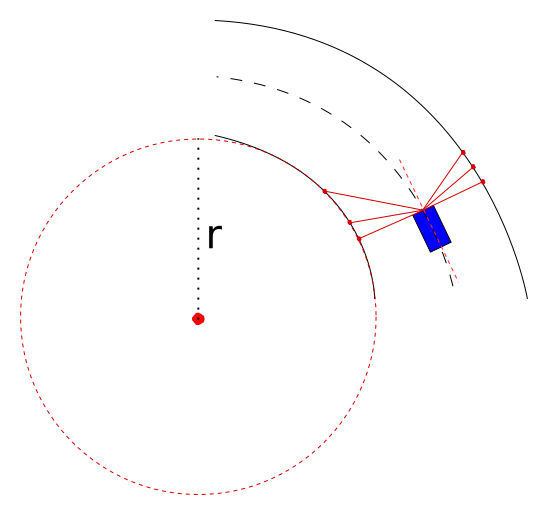
\includegraphics[width=0.8\columnwidth]{Curvature.pdf}}
\caption{Curvature of the track line extrapolated from three points measured in the sensor space.}
\label{fig-curvature}
\end{figure}

In practice, this yields results that are off by a slight error margin for every track. The data is only as good as the readings, and keeping the car running at a pace that will not get it disqualified by the game (and thus instantly removed from the track), while getting steady readings is not always possible. As such, we do minor corrections to the data after recording the track. The biggest change is making sure that the collective angles of all the points sum up to 360 degrees, as all tracks in TORCS begin and end in the same point.

\subsection{Euclidean Representation}
\subsubsection{Construction}
The track data from the warm-up period contains a set of track points $D$ in the sensor space, which are all assumed to fall on the track line. A single point $d_i \in D$ has a payload of 4 values:
\begin{itemize}
\item its distance from the start line $|d_0 d_i|$ (equivalent to the arc length of the track line segment between $d_0$ and $d_i$)
\item the angle $d_i \angle d_{i+1}$ between the tangent to the track at $d_i$ and at the following point $d_{i+1}$
\item the width of the road $w^+(d_i)$ in the positive direction
\item the width of the road $w^-(d_i)$ in the negative direction
\end{itemize}

Using this data, it is possible to map the track to a representation in Euclidean space. This approach involves mapping $d_0$ to the origin $(0,0)$, and then displacing every following Euclidean point $p_i$ by the angle and distance from $d_i$ to $d_{i+1}$, thus obtaining the coordinates for $p_{i+1}$.

This workflow is illustrated in algorithm \ref{alg-tmc}, where the track model is constructed by assigning to the functions $D(x)$ and $P(d_x)$ (lines \ref{line-dx} and \ref{line-px}), where $D(x)=d_x \Rightarrow x=|d_0 d_x|$ and $P(d_x)$ yields the Euclidean point $p$ corresponding to the track point $d_x$.

\begin{algorithm}
\caption{Track Model Construction}
\label{alg-tmc}
\begin{algorithmic}[1]
\State $p \gets (0,0)$
\ForAll{$d_0..d_{n-1} \in D$}
	\State $l \gets |d_i d_{i+1}|$
	\State $\alpha \gets d_0 \angle d_{i+1}$
	\State $\vec{v} \gets \vect{l & \cos{\alpha}}{l & \sin{\alpha}}$
	\State $p \gets p+\vec{v}$
	\State $D(|d_0 d_i|) \gets d_i$ \label{line-dx}
	\State $P(d_i) \gets p$ \label{line-px}
\EndFor
\end{algorithmic}
\end{algorithm}

\subsubsection{Transformation}
\label{sec-trans}
We wish to distinguish between states in the sensor space and those in the Euclidean space. We define a state $\sigma$ as being represented in the sensory model, and a state $s$ as being represented in the vector model. An action $a$ can be applied to either representation in order to advance the game.\footnote{Note that applying an action $a$ to a state $\sigma$ is only possible in real-time by actually taking that action in the game. Simulations require the use of the vector space representation and forward model.}

A state $\sigma$ represents a subset of data from the sensory data model from \cite{manual}, named as follows:
\begin{itemize}
\item $\delta$ -- distance from start along the track line (m)
\item $\tau$ -- normalized distance to the closest point on the track line ($[-1;1]$)
\item $\theta$ -- angle between the yaw of the car and the gradient of the track line at the closest point (radians)
\item $\gamma$ -- speed of the car in the direction of its yaw (km/h)
\end{itemize}

Note the absence of lateral velocity. Between actions, we always consider states to be quiescent, having no acceleration and no lateral velocity.\footnote{This allows us to keep the transformation logic strictly concerned with states, and the forward model strictly concerned with the application of actions to states. Acceleration and lateral velocity is related to gas and steering, both components of actions, the exclusive domain of the forward model.}

A state $s$ is represented by the following two components:
\begin{itemize}
\item the position of the car, given as a point $p=(x,y)$
\item the velocity of the car, given as a vector $\vec{v}$
\end{itemize}

A state $\sigma$ and a state $s$ is related by the functions in equation (\ref{eqn-transforms}), allowing us to transform a representation in the sensory model to one in the vector model, and vice versa.

\begin{equation}
\begin{alignedat}{1}
\label{eqn-transforms}
T_v (\sigma) = s \\
T_s (s) = \sigma
\end{alignedat}
\end{equation}

Theoretically, reflexivity (\ref{eqn-tref}) is intended to hold for the above definitions. Note, however, that our internal model can only approximate this relation, so there is a slight loss of accuracy when performing the transformations in practice. See section \ref{sec-accuracy} for measurements of this error.

\begin{equation}
\begin{alignedat}{1}
\label{eqn-tref}
T_v (T_s (s)) \approx s \\
T_s (T_v (\sigma)) \approx \sigma
\end{alignedat}
\end{equation}

Algorithms \ref{alg-tv} and \ref{alg-ts} display in pseudo-code the implementations of these functions, where the symbols $\delta, \tau, \theta, \gamma$ for states $\sigma$ and $p, \vec{v}$ for states $s$ are used as defined above.

Thus, lines \ref{line-ass-p} and \ref{line-ass-v} of algorithm \ref{alg-tv} assign to a new state $s$, where lines \ref{line-ass-delta}, \ref{line-ass-theta}, \ref{line-ass-gamma}, \ref{line-ass-tau1} and \ref{line-ass-tau2} of algorithm \ref{alg-ts} assign to a new state $\sigma$.

At line \ref{line-det} of algorithm \ref{alg-ts}, the vector determinant is used to find the orientation of $p$ relative to the track line (left- or right-hand side). This is analogous to using the cross-product in 3-dimensional space \cite{crossp} for the same purpose.

\begin{algorithm}
\caption{Transformation $T_v$}
\label{alg-tv}
\begin{algorithmic}[1]
\State $\alpha \gets D(0) \angle D(\delta)$
\If{$\tau > 0$}
	\State $t \gets \tau * w^+(D(\delta))$
\Else
	\State $t \gets \tau * w^-(D(\delta))$
\EndIf
\State $p \gets P(D(\delta))+\vect{t & \cos{\alpha}}{t & \sin{\alpha}}^\bot$ \label{line-ass-p} \Comment{Perpendicular vector}
\State $\vec{v} \gets \vect{\gamma / 3.6}{0}+\alpha+\theta$ \label{line-ass-v} \Comment{Conversion to m/s}
\end{algorithmic}
\end{algorithm}

\begin{algorithm}
\caption{Transformation $T_s$}
\label{alg-ts}
\begin{algorithmic}[1]
\State $d_x \gets P^-(p)$ \Comment{Inverse of function P (closest track point to $p$)}
\State $\delta \gets |d_0 d_x|$ \label{line-ass-delta}
\State $\theta \gets \angle\vec{v} - d_0 \angle d_x$ \label{line-ass-theta}
\State $\gamma \gets |\vec{v}| * 3.6$ \label{line-ass-gamma} \Comment{Conversion to km/h}
\State $m \gets P(d_x)$
\State $n \gets P(d_{x+1})$
\If{$det(\vec{mn},\vec{mp}) > 0$} \Comment {Vector determinant} \label{line-det}
	\State $\tau \gets |mp| / w^+(d_x)$ \label{line-ass-tau1}
\Else
	\State $\tau \gets -|mp| / w^-(d_x)$ \label{line-ass-tau2}
\EndIf
\end{algorithmic}
\end{algorithm}

\subsection{Forward Model}

Equation (\ref{eqn-fstep}) displays the forward step function, which takes a state $s$ in the vector model and applies an action $a$ to it, yielding a state $s'$, which represents $s$ projected a fixed time interval into the future, with the car having held the same $a_{gas}$ and $a_{steering}$ for the duration of the interval.

\begin{equation}
\label{eqn-fstep}
F(s,a)=s'
\end{equation}

The implementation of the forward step function relies on assumptions about the relationship between pressure on the gas pedal and acceleration, and between rotation of the steering wheel and angular velocity. We have approximated these relationships through experimentation and regression analysis on recorded sets of data.

\subsubsection{Gas}
The relationship between pressure on the gas pedal and acceleration of the car is dependent on various physical properties of the car and thus data from the given car is needed in order to construct a model of the relationship. To gather this data, a track with a long straight stretch is needed for high speeds. A simple controller, that keeps constant gas pressure while changing gears at high RPM, is driven down the stretch while recording data about its speed, gear and acceleration. At the end of the stretch the controller resets itself and runs again with a different gas pressure.

A custom script for RapidMiner \cite{rapidminer} was used to do regression analysis on the data, to produce an equation for each interval of gear and gas, totaling 42 equations with 6 gears and 10 different gas intervals. Higher gear levels do not have data with low throttle as this makes it impossible to reach those gears. The equations are indexed after gas and gear so that they can be accessed by the controller. If the controller requests an equation that does not exist, an equation with a lower gas pressure is used instead. As data was only collected for accelerating speeds, any form of deceleration will be inaccurate. How this affects the controller is discussed in section \ref{sec-discussion}.

\subsubsection{Steering}
To model the relationship between velocity, steering and the car's future position in Euclidean space, it is convenient to apply the concept of \emph{angular velocity} \cite{angv}\cite{rotq}. Through experimentation, we found that the steering property of an action in TORCS, together with the car's current speed, is directly related to the radius $r$ of the circle around which the car will rotate (drawing it to the side as it travels forward). The steering is inversely proportional to the radius (the more steering, the smaller the circle along which the rotation happens), while the speed is directly proportional (the higher the speed, the bigger the circle). Equation (\ref{eqn-steering}) displays our radius approximation function $R(a_s,\bar{v})$. The values for the formula have been assigned by regression analysis on experimental data.

\begin{equation}
\label{eqn-steering}
R(a_s,\bar{v})=176.8927*0.000272^{|a_s|}*1.0099^{\bar{v}}
\end{equation}
where $a_s$ is the steering property of the action $a$ and $\bar{v}$ is the average velocity of the car in the given forward step.

Equation (\ref{eqn-angv}) displays the formula we use to determine angular velocity, where $r$ is the radius, $\bar{v}$ is the velocity in m/s, $\omega$ is the angular velocity (radians/s) and $\theta$ is the angular distance travelled (radians) around a circle of size $r$ in $t$ seconds, $t$ being the time interval of the forward step.

\begin{equation}
\label{eqn-angv}
\begin{alignedat}{1}
& r = R(a_s,\bar{v}) \\
& \omega = \bar{v} / r \\
& \theta = \omega * t
\end{alignedat}
\end{equation}

In practice, steering is limited by other factors such as road grip, causing the car to skid if it attempts sharp turns at high velocities. This is a shortcoming of our model.

\subsection{Model Accuracy and Performance}
\label{sec-accuracy}

In order to properly review the performance of our car controller, it is important first to establish the impact of our simulation framework on the accuracy of the controller's decision-making. As stated in section \ref{sec-trans}, the transformations between states in the sensor model and vector model are off by a slight margin of error. We have measured this error, as shown in table \ref{tab-accuracy}. The second column displays the average discrepancy between the input state $\sigma$ and output state $\sigma'$ for the given sensor after the transformation $T_s(T_v(\sigma))=\sigma'$, measured every tick for 5 seconds, totalling 250 measurements. During our tree search, states are not transformed back and forth multiple times, so a discrepancy of just 5 centimeters is acceptable, and unlikely to be the cause of suboptimal benchmarks of the controller as a whole.

Table \ref{tab-performance} gives an idea of how much of an impact our simulation framework has on the runtime performance of our tree search algorithm. It compares the number of iterations possible with a timeout of 10 milliseconds on an isolated tree search with no simulation framework being invoked, to the same benchmark with transformations and/or forward stepping being applied in the search. It can be seen that having the full framework present cuts the number of iterations to 43\% compared to its absence.

\begin{table}
\begin{center}
\renewcommand{\arraystretch}{1.3}
\caption{Average Transformation Error}
\label{tab-accuracy}
\begin{tabular}{|c|c|} \hline
\textbf{Sensor} & \textbf{Avg. discrepancy} \\ \hline
Distance from start & $0.053$ m \\ \hline
Track position & $0.027$ m \\ \hline
Angle to track & $2.2*10^{-5}$ radians \\ \hline
\end{tabular}
\end{center}
\end{table}

\begin{table}
\begin{center}
\renewcommand{\arraystretch}{1.3}
\caption{Simulation Framework Performance Impact}
\label{tab-performance}
\begin{tabular}{|c|c|c|} \hline
\textbf{Measurement} & \textbf{No. of iterations} & \textbf{Fraction} \\ \hline
Isolated tree search & $1937.7$ & 100\% \\ \hline
Only transformation & $1413.8$ & 73\% \\ \hline
Only forward step & $1242.3$ & 64\% \\ \hline
Full framework & $842.2$ & 43\% \\ \hline
\end{tabular}
\end{center}
\end{table}

\section{Results}
\label{sec-results}

In this paper, we are comparing ourselves to the competitions held in 2008 \cite{2008championship} and 2009 \cite{2009championship}. Figure \ref{fig-scores} displays how our own controller, labelled Fischer-Falsted-Vielwerth, compares to the results from those years. For the competition, a set of three tracks is selected and each controller is run ten times on each track for 10,000 game ticks. The median of the distance raced is then used as a score. We were unfortunately unable to use results from later competitions, as they are run on generated tracks rather than the default TORCS tracks.

The three selected tracks in the 2008 competition consist of one hill track, one tarmac track, and one oval track. For the 2009 competition, the tracks consist of one hill track, one dirt track and one tarmac track. As our forward model is based on data from tarmac tracks, we are unable to compete on dirt and hill tracks. Our scores were consistently lowest on those tracks, so we have omitted them from our charts.

Compared to the 2008 controllers, we make first place on Street-1 and hit the top three on Speedway. The 2009 controllers drive significantly better, so we only achieve scores comparable to the bottom three controllers.

\begin{figure*}
\caption{2008 and 2009 competition benchmarks}
\label{fig-scores}
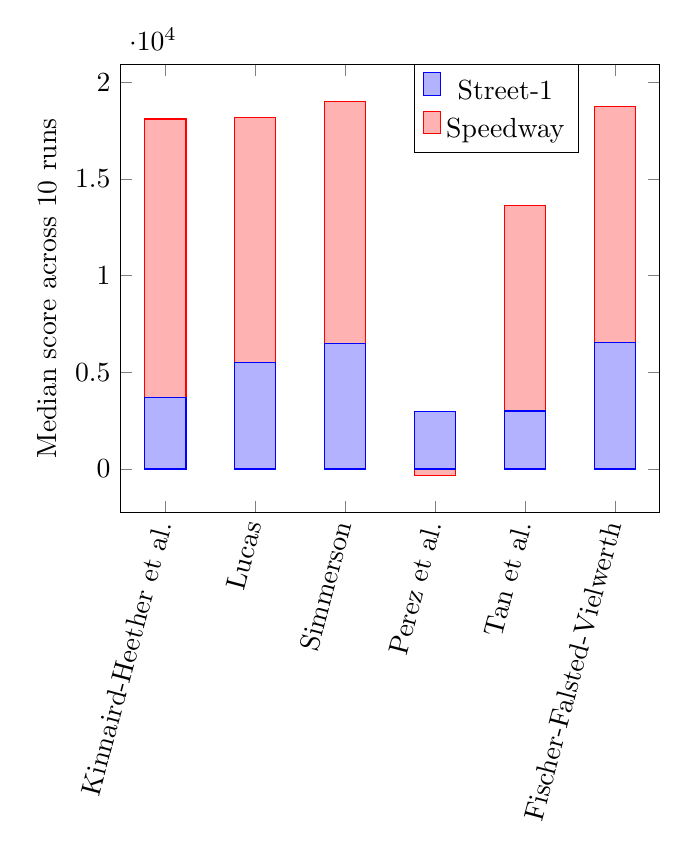
\begin{tikzpicture}
\begin{axis}[ybar stacked, bar width=15pt, ylabel={Median score across 10 runs}, symbolic x coords={
	Kinnaird-Heether et al., Lucas, Simmerson, Perez et al., Tan et al., Fischer-Falsted-Vielwerth
}, xtick=data, x tick label style={rotate=75, anchor=east}, legend style={at={(0.85, 1.0)}}]
\addplot+[ybar] plot coordinates {
	(Kinnaird-Heether et al., 3692.9)
	(Lucas, 5502.8)
	(Simmerson, 6477.8)
	(Perez et al., 2984.8)
	(Tan et al., 2998.5)
	(Fischer-Falsted-Vielwerth, 6559.4)
};
\addplot+[ybar] plot coordinates {
	(Kinnaird-Heether et al., 14406.9)
	(Lucas, 12664.5)
	(Simmerson, 12523.3)
	(Perez et al., -317.3)
	(Tan et al., 10648.2)
	(Fischer-Falsted-Vielwerth, 12201.4)
};
\legend{\strut Street-1, \strut Speedway}
\end{axis}
\end{tikzpicture}
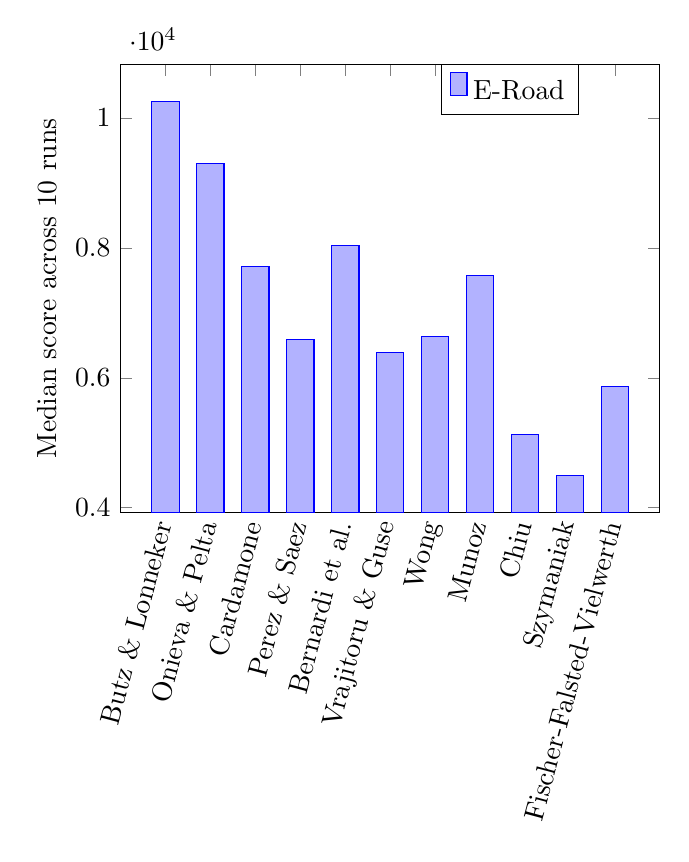
\begin{tikzpicture}
\begin{axis}[ybar stacked, bar width=10pt, ylabel={Median score across 10 runs}, symbolic x coords={
	Butz \& Lonneker, Onieva \& Pelta, Cardamone, Perez \& Saez, Bernardi et al., Vrajitoru \& Guse,
	Wong, Munoz, Chiu, Szymaniak, Fischer-Falsted-Vielwerth
}, xtick=data, x tick label style={rotate=75, anchor=east}, legend style={at={(0.85, 1.0)}}]
\addplot+[ybar] plot coordinates {
	(Butz \& Lonneker, 10253.3)
	(Onieva \& Pelta, 9301.1)
	(Cardamone, 7716.3)
	(Perez \& Saez, 6586.6)
	(Bernardi et al., 8036.8)
	(Vrajitoru \& Guse, 6384.4)
	(Wong, 6638.3)
	(Munoz, 7573.5)
	(Chiu, 5124.3)
	(Szymaniak, 4501.7)
	(Fischer-Falsted-Vielwerth, 5865.4)
};
\legend{\strut E-Road}
\end{axis}
\end{tikzpicture}
\end{figure*}

\section{Discussion}
\label{sec-discussion}

Our controller competes well on tarmac roads, and by fine-tuning the configurable constants we saw an increase in our controller's performance on the benchmarks. The driving behaviour observed align in some cases with human behavior, such as accelerating on straight sections and braking before turns, compared to earlier in the project, where driving speed was generally limited by the lowest speed possible on the track.

The three tracks chosen for the competitions usually contain at least one track that is either a dirt track or a hill track. A dirt track has low traction, which causes high speed on acceleration to spin or skid the car. A hill track has steep climbs and descends, making the car accelerate slower or faster than on a flat track. Both these types changes the basic premises for how the car handles on the track. Since this is not part of the calculations in our forward model, we are at this point unable to race these tracks at competitive speeds. In the future, changes to the forward model together with tests of traction during the warm-up is likely to let us achieve results on dirt and hill tracks, similar to those obtained on tarmac. A further improvement would be to collect actual data about how the car brakes, instead of the hand tuned solution that describes deceleration at the moment.

As we have limited the amount of actions to not contain heavy braking and steering at the same time, positioning of the car before a corner plays an important role. Having the car on the wrong side of the track before a corner forces the car to change position before being able to hit the brake. This can lead to anything, from not taking the corner optimally to not taking the corner at all. An example of this is how the car handles turn 11 on the Street 1 track. Turn 11 is a very sharp hairpin. The speed of the car needs to be very low, but the turn ends the longest straight on the track. The time it takes to brake is therefore high, as it enters the braking zone at high speed. If the car is not positioned well when the search reaches the upcoming turn, it needs to adjust its position to make a proper entry. The time it takes to make this adjustment makes it unable to complete the deceleration in time, and the car either comes to a complete halt or leaves the road. We attribute this behavior to the relatively low depth of the search tree. With a greater depth, the controller might realize that the turn is coming up sooner, thus repositioning the car before entering the brake zone.

Since the focus of this project has been to implement and test Monte-Carlo Tree Search, we decided not to augment the controller with special case handling such as ABS (Anti-lock braking system), ESP (Electronic stability program) and off track recovery. These augmentations would likely have increased our scores, but we felt it would pollute the results of the actual tree search, overshadowing potential faults.

\section{Future Work}
\label{sec-futurework}
While we feel that MCTS and/or other model-based approaches have their merit in terms of providing the controller with a mechanism for planning its decisions, it cannot stand entirely on its own. In particular, the forward model is far too fragile if hard-coded, which is the current state of the solution presented in this article. A learned forward model based on data directly from the sensor space was obtained by Butz et al. \cite{cobostar}, and we expect a similar approach could succeed in learning a forward model that would apply instead in the reconstructed track model.

A learned forward model provides an abstraction of the underlying engine with much better potential for accuracy and efficiency. The biggest advantage is likely its generalizability, which is of paramount importance with respect to different track types. The rules governing the relationship between the controller’s actions and the car’s behaviour in the game world can be radically different (e.g. road tracks vs. dirt tracks), and a forward model that can adapt to these differences seems like a fundamental ingredient in any model-based approach.

For this purpose, it may be beneficial to apply a certain measure of active learning, either during warm-up or in the actual race. The controller cannot know beforehand which kind of track it is about to race on, but a sophisticated implementation to could learn during the race which of its pre-trained forward models apply. A similar approach might have a pre-trained forward model representing the “lowest common denominator” between all tracks, which is then gradually reinforced to model a particular track as the actual race progresses.

\section{Conclusions}
\label{sec-conclusion}
Throughout this paper, we have presented our work with Monte-Carlo Tree Search in the TORCS racing game. The tree search is tuned to maximize the distance raced within the allotted time. We can successfully build a track model and perform simulations in it, but the forward model used to simulate these steps was found, under certain circumstances, to have deficiencies compared to what actually plays out. We attained better driving capabilities by pruning the action space and removing actions with outcomes known to be undesirable. The implementation fares good compared to results from 2008 and 2009, but fails when driving on dirt or hill tracks, as the forward model is optimized for tarmac roads. By looking at the scores compared to the other controllers, we find that Monte-Carlo Tree Search or similar model-based approaches may present a viable option for controlling racing cars at competetive speeds.

\begin{savenotes}
\begin{table}
\begin{center}
\renewcommand{\arraystretch}{1.3}
\caption{Configurable constants}
\label{tab-config}
\begin{tabular}{|c|c|} \hline
\multicolumn{2}{c}{General} \\ \hline
Decision time step [$s$] & 0.25 \\ \hline
Timeout [$ms$] & 15 \\ \hline
Gear limit\footnote{Gear limit is set to 2 on the Street-1 track.} & 2/6 \\ \hline
\multicolumn{2}{c}{Evaluation} \\ \hline
Off course boundary & 5.3 \\ \hline
Off track boundary & 0.7 \\ \hline
Penalty factor & 0.4 \\ \hline
Max. acceleration [$m/s^2$] & 10 \\ \hline
\multicolumn{2}{c}{Monte-Carlo} \\ \hline
$C_P$ value & 0.7 \\ \hline
Simulation depth limit & 3 \\ \hline
\multicolumn{2}{c}{Action Space Definition} \\ \hline
Gas interval size & 0.2 \\ \hline
Steering interval size & 0.1 \\ \hline
Gas discretization factor & 5 \\ \hline
Steering discretization factor & 10 \\ \hline
\end{tabular}
\end{center}
\end{table}
\end{savenotes}

\begin{thebibliography}{22}
\bibitem{torcs}
B.~Wymann, ``TORCS, The Open Racing Car Simulator". http://torcs.sourceforge.net/

\bibitem{manual}
D.~Loiacono, L.~Cardamone, P.~L.~Lanzi, ``Simulated Car Racing Championship Competition Software Manual", April 2013.

\bibitem{browne}
C.~Browne, E.~Powley, D.~Whitehouse, S.~Lucas, P.~I.~Cowling, P.~Rohlfshagen, S.~Tavener, D.~Perez, S.~Samothrakis, and S.~Colton, ``A Survey of Monte Carlo Tree Search Methods", \emph{IEEE Transactions on Computational Intelligence and AI in Games}, 2012, pp. 1--49.

\bibitem{2008championship}
D.~Loiacono, J.~Togelius, P.~L.~Lanzi, L.~Kinnaird-Heether, S.~M.~Lucas, M.~Simmerson, D.~Perez, R.~G.~Reynolds, and Y.~Saez, ``The WCCI 2008 Simulated Car Racing Competition", \emph{IEEE Symposium on Computational Intelligence and Games}, 2008, pp. 119--126.

\bibitem{2009championship}
D.~Loiacono, P.~Lanzi, J.~Togelius, E.~Onieva, D.~Pelta, M.~Butz, T.~Lönneker, L.~Cardamone, D.~Perez, Y.~Sáez, M.~Preuss, and J.~Quadflieg, ``The 2009 Simulated Car Racing Championship", \emph{IEEE Transactions on Computational Intelligence and AI in Games}, 2009, pp. 131--147.

\bibitem{optimalraceline}
L.~Cardamone, D.~Loiacono, P.~Lanzi, and A.~Bardelli, ``Searching for the optimal racing line using genetic algorithms", \emph{IEEE Symposium on Computational Intelligence and Games}, 2010, pp. 388--394.

\bibitem{trackmodel}
J.~Quadflieg, M.~Preuss, O.~Kramer, and G.~Rudolph, ``Learning the track and planning ahead in a car racing controller", \emph{IEEE Symposium on Computational Intelligence and Games}, 2010, pp. 395--402.

\bibitem{cobostar}
M.~Butz and T.~Lonneker, ``Optimized Sensory-motor Couplings plus Strategy Extensions for the TORCS Car Racing Challenge", \emph{IEEE Symposium on Computational Intelligence and Games}, 2010, pp. 317--324.

\bibitem{fluff}
N.~van Hoorn, J.~Togelius, D.~Wierstra, and J.~Schmidhuber, ``Robust player imitation using multiobjective evolution", \emph{IEEE Congress on Evolutionary Computation}, 2009, pp. 652--659.

\bibitem{go}
A.~Rimmel, F.~Teytaud, L.~Chang-Shing, Y.~Shi-Jim, W.~Mei-Hui, and T.~Shang-Rong, ``Current Frontiers in Computer Go", \emph{IEEE Transactions on Computational Intelligence and AI in Games}, 2010, pp. 229--238.

\bibitem{hex}
B.~Arneson, R.~B.~Hayward, and P.~Henderson, ``Monte-Carlo tree search in Hex", \emph{IEEE Transactions on Computational Intelligence and Games}, 2010, pp. 251--258.

\bibitem{pacman}
T.~Pepels and M.~H.~M.~Winands, ``Enhancements for Monte-Carlo Tree Search in Ms Pac-Man", \emph{IEEE Conference on Computational Intelligence and Games}, 2012, pp. 265--272.

\bibitem{raceline}
B.~Beckman, ``The Physics of Racing, Part 5: Introduction to the Racing Line", 1991. http://www.miata.net/sport/Physics/05-Cornering.html

\bibitem{euclidean}
S.~Christopher, and E.~W.~Weisstein, ``Euclidean Space", \emph{MathWorld}--A Wolfram Web Resource. http://mathworld.wolfram.com/EuclideanSpace.html

\bibitem{circle}
E.~W.~Weisstein, ``Circumcircle", \emph{MathWorld}--A Wolfram Web Resource. http://mathworld.wolfram.com/Circumcircle.html

\bibitem{curve}
E.~W.~Weisstein, ``Curvature", \emph{MathWorld}--A Wolfram Web Resource. http://mathworld.wolfram.com/Curvature.html

\bibitem{crossp}
E.~W.~Weisstein, ``Cross Product", \emph{MathWorld}--A Wolfram Web Resource. http://mathworld.wolfram.com/CrossProduct.html

\bibitem{angv}
E.~W.~Weisstein, ``Angular Velocity", \emph{MathWorld}--A Wolfram Web Resource. http://mathworld.wolfram.com/AngularVelocity.html

\bibitem{motion}
R.~Nave, ``Description of Motion", \emph{HyperPhysics}--Department of Physics and Astronomy, Georgia State University. http://hyperphysics.phy-astr.gsu.edu/hbase/mot.html

\bibitem{rotq}
R.~Nave, ``Rotational Quantities", \emph{HyperPhysics}--Department of Physics and Astronomy, Georgia State University. http://hyperphysics.phy-astr.gsu.edu/hbase/rotq.html

\bibitem{simplix}
``TORCS Robot Development | Simplix". http://www.simplix.wdbee-aorp.de/SIMPLIX/SimplixDefault.aspx

\bibitem{rapidminer}
``RapidMiner". https://rapidminer.com/
\end{thebibliography}

\newpage

\begin{appendices}
\section{Track Definition Example}
\label{apx-track}
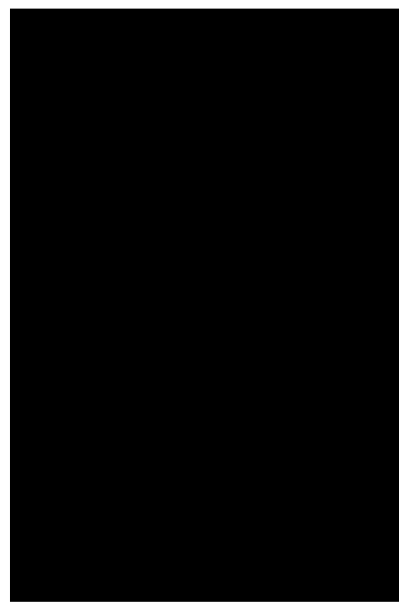
\includegraphics[width=\columnwidth]{trackdef.pdf}

\section{TORCS Setup Guide}
Download and install TORCS 1.3.4 for Windows.\\
\textbf{https://sourceforge.net/projects/torcs/files/torcs-win32-bin/}

Download the patch files and copy them into the TORCS folder. Overwrite any conflicting files.\\
\textbf{http://sourceforge.net/projects/cig/files/SCR\%20Championship/Server\%20Windows/2.0/patch.zip/download}

Dowload the controller that acts as a UDP server. Copy the content into the drivers subfolder.\\
\textbf{http://sourceforge.net/projects/cig/files/SCR\%20Championship/Client\%20Java/2.0/scr-client-java.tgz/download}

Further instructions can be found at \textbf{http://arxiv.org/pdf/1304.1672.pdf}

\section{Video}
A short video showing how the controller handles a track and how it gathers data about the track.\\
\textbf{https://www.youtube.com/watch?v=rKcSIDMPoVg}
\end{appendices}
\end{document}
